\documentclass[12pt]{article}

% ========== PACKAGES ==========
\usepackage{amsmath}
\usepackage{amssymb}          % For math symbols
\usepackage{graphicx}         % To include images
\usepackage[a4paper, margin=1in]{geometry} % For page layout
\usepackage{xcolor}           % For colors
\usepackage{hyperref}         % For hyperlinks
\usepackage{fancyhdr}         % For headers and footers
\usepackage{titling}          % <--- CRITICAL FIX: Allows usage of \thetitle
\usepackage{tikz}             % For drawing diagrams
\usepackage{siunitx}          % For typesetting units correctly
\usepackage{gensymb}          % Provides \degree

% ========== TIKZ LIBRARIES ==========
\usetikzlibrary{decorations.pathmorphing}
\usetikzlibrary{arrows.meta}

% ========== DOCUMENT INFORMATION ==========
\title{Teaching Notes \& Solved Problems: Thermal Conductivity}
\author{Physics Dept.}
\date{\today}

% ========== HEADER AND FOOTER ==========
\pagestyle{fancy}
\fancyhf{}
\rhead{Thermal Conductivity}
\lhead{\thetitle}             % This will now work because of 'titling' package
\cfoot{\thepage}

\begin{document}

\maketitle
\thispagestyle{empty}
\tableofcontents
\newpage

\section{Teaching Notes: Thermal Conductivity (1-Hour Lesson)}

\subsection{Part 1: The Basics of Heat Conduction (15 mins)}

\subsubsection*{What is Heat Conduction?}
Heat conduction is the transfer of thermal energy through a substance by the collision of its constituent particles (atoms, molecules, electrons).
\begin{itemize}
    \item In \textbf{solids}, atoms vibrate in fixed positions and pass energy to their neighbors. In metals, free-moving electrons also carry energy, making them excellent conductors.
    \item Conduction is one of the three modes of heat transfer, along with \textbf{convection} (heat transfer by fluid movement) and \textbf{radiation} (heat transfer by electromagnetic waves).
\end{itemize}

\subsubsection*{Fourier's Law of Heat Conduction}
The fundamental equation for heat conduction is Fourier's Law. For a uniform object like a rod, the rate of heat flow ($P$) is given by:
\begin{equation}
    P = \frac{dQ}{dt} = \frac{kA(T_H - T_C)}{L}
\end{equation}
Let's break down the terms:
\begin{itemize}
    \item \textbf{$P$}: The \textbf{rate of heat flow} (heat current), in \si{\watt} (or \si{\joule\per\second}).
    \item \textbf{$k$}: The \textbf{thermal conductivity}, in \si{\watt\per\meter\per\kelvin}.
    \item \textbf{$A$}: The \textbf{cross-sectional area}, in \si{\meter\squared}.
    \item \textbf{$T_H$} and \textbf{$T_C$}: The temperatures of the \textbf{hot} and \textbf{cold} ends.
    \item \textbf{$L$}: The \textbf{length} of the material, in \si{\meter}.
\end{itemize}

% Diagram of Heat Conduction
\begin{figure}[h!]
\centering
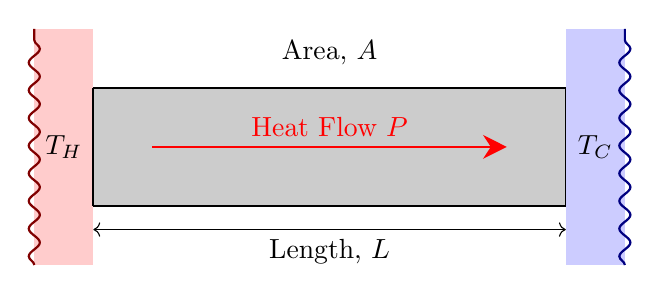
\begin{tikzpicture}[scale=1.5]
    % Hot Reservoir
    \fill[red!20] (-0.5, -1) rectangle (0, 1);
    \draw[red!50!black, thick, decoration={snake, segment length=10pt, amplitude=2pt}, decorate] (-0.5, -1) -- (-0.5, 1);
    \node at (-0.25, 0) {$T_H$};
    
    % Rod
    \fill[gray!40] (0, -0.5) rectangle (4, 0.5);
    \draw[thick] (0, -0.5) -- (4, -0.5);
    \draw[thick] (0, 0.5) -- (4, 0.5);
    \draw[thick] (0, -0.5) -- (0, 0.5);
    \draw[thick] (4, -0.5) -- (4, 0.5);

    % Heat Flow Arrow
    \draw[-{Stealth[length=3mm, width=3mm]}, red, thick] (0.5, 0) -- (3.5, 0) node[midway, above] {Heat Flow $P$};
    
    % Cold Reservoir
    \fill[blue!20] (4, -1) rectangle (4.5, 1);
    \draw[blue!50!black, thick, decoration={snake, segment length=10pt, amplitude=2pt}, decorate] (4.5, -1) -- (4.5, 1);
    \node at (4.25, 0) {$T_C$};
    
    % Labels
    \draw[<->] (0, -0.7) -- (4, -0.7) node[midway, below] {Length, $L$};
    \node at (2, 0.8) {Area, $A$};
\end{tikzpicture}
\caption{Heat conduction through a uniform rod.}
\label{fig:conduction}
\end{figure}

\subsection{Part 2: Applying the Concept (15 mins)}

\subsubsection*{Connecting to Other Thermal Concepts}
The heat ($Q$) transferred by conduction can cause:
\begin{enumerate}
    \item \textbf{Phase Changes (Latent Heat):} To change a substance's state (e.g., melt ice) at a constant temperature.
    \[ Q = m L_{\mathrm{f}} \]
    The rate of mass melting is related to the rate of heat flow: $P = \frac{dQ}{dt} = L_f \frac{dm}{dt}$.

    \item \textbf{Temperature Changes (Specific Heat Capacity):} To change a substance's temperature.
    \[ Q = mc\Delta T \]
\end{enumerate}

\newpage
\section{Solutions to Provided Problems}

\subsection{Problem 1 (SPhO 2022)}
\subsubsection*{Solution (i): Thermal Conductivity}
\begin{enumerate}
    \item \textbf{Calculate rate of heat flow ($P$)}:
    \[ \frac{dm}{dt} = \SI{0.1683}{\kilogram\per\minute} \times \frac{1}{60} = \SI{0.002805}{\kilogram\per\second} \]
    \[ P = L_f \frac{dm}{dt} = (\SI{3.36e4}{}) (\SI{0.002805}{}) = \SI{94.248}{\watt} \]
    
    \item \textbf{Solve for $k$}:
    Given $L = \SI{0.200}{\meter}$, $r = \SI{0.0100}{\meter}$, $\Delta T = \SI{150}{\kelvin}$.
    \[ A = \pi r^2 = \pi (\SI{0.0100}{})^2 \approx \SI{3.14e-4}{\meter\squared} \]
    \[ k = \frac{PL}{A\Delta T} = \frac{(94.248)(0.200)}{(\pi \times 10^{-4})(150)} \approx \SI{400}{\watt\per\meter\per\kelvin} \]
\end{enumerate}

\subsubsection*{Solution (ii): Rate of Entropy Change}
Temperatures in Kelvin: $T_H = \SI{423.15}{\kelvin}$, $T_C = \SI{273.15}{\kelvin}$.
\begin{itemize}
    \item Hot Source: $\frac{dS}{dt} = \frac{-94.248}{423.15} = \SI{-0.2227}{\joule\per\kelvin\per\second}$
    \item Cold Source: $\frac{dS}{dt} = \frac{+94.248}{273.15} = \SI{+0.3451}{\joule\per\kelvin\per\second}$
    \item \textbf{Total}: $\SI{0.1224}{\joule\per\kelvin\per\second}$
\end{itemize}

\end{document}
